\chapter{Treatment System}
\label{ch:treatment}

These genetic mutations create vulnerabilities that treatments can exploit. This chapter examines exactly how immune checkpoint inhibitors and targeted therapies work --- and reveals why the ICI+TKI combination is more than the sum of its parts.

This chapter describes the pharmacological treatment layer of the model, which simulates Immune Checkpoint Inhibitors (ICI), Tyrosine Kinase Inhibitors (TKI), and their combination. The treatment system is activated after a configurable number of simulation steps and modulates tumor and immune cell behaviors through drug-specific mechanisms.

%% ====================================================================
\section{Drug Architecture}
\label{sec:drug-architecture}

\begin{figure}[htbp]
\centering
\adjustbox{max width=0.85\textwidth, max height=0.7\textheight}{% Treatment Mechanisms: ICI, TKI, and Synergy — 3 stacked panels
\begin{tikzpicture}[
    drug/.style={rectangle, rounded corners=3pt, draw, fill=treatment!80, text=white,
                 font=\small\bfseries, minimum height=0.6cm, inner sep=4pt},
    cell/.style={circle, draw, minimum size=0.7cm, font=\small\bfseries, inner sep=0pt},
    effect/.style={rectangle, rounded corners=3pt, draw, fill=treatment!15,
                   font=\small, inner sep=4pt},
    panellabel/.style={font=\small\bfseries, anchor=west},
    arrow/.style={->, >=stealth, thick}
]

% ── Panel 1: ICI ──────────────────────────────────────────────
\node[panellabel] at (0,9.2) {Panel A: Immune Checkpoint Inhibition (ICI)};
\draw[neutral, thick] (0,8.9) -- (13,8.9);

\node[cell, fill=immunecell!25] (tcell) at (1.5,7.8) {T};
\node[font=\footnotesize, anchor=south] at (1.5,8.2) {T Cell};

% PD-1/PD-L1 bridge
\draw[thick, red, <->] (2.2,7.8) -- (3.8,7.8)
    node[midway, above, font=\footnotesize] {PD-1/PD-L1};

\node[cell, fill=tumorcell!25] (tumour1) at (4.5,7.8) {TC};
\node[font=\footnotesize, anchor=south] at (4.5,8.2) {Tumor};

% ICI drug breaking the connection
\node[drug] (ici) at (3,6.6) {ICI};
\draw[arrow, treatment] (ici) -- (3,7.55)
    node[midway, right, font=\footnotesize] {blocks};

% X through the bridge
\draw[red, very thick] (2.7,7.5) -- (3.3,8.1);
\draw[red, very thick] (2.7,8.1) -- (3.3,7.5);

% Outcome
\draw[arrow] (5.3,7.8) -- (7.2,7.8);
\node[effect] (ici_out) at (9.5,7.8) {Restored T Cell Killing};

% ── Panel 2: TKI ──────────────────────────────────────────────
\node[panellabel] at (0,5.9) {Panel B: Tyrosine Kinase Inhibition (TKI)};
\draw[neutral, thick] (0,5.6) -- (13,5.6);

\node[cell, fill=tumorcell!25] (tumour2) at (1.5,4.5) {TC};
\node[font=\footnotesize, anchor=south] at (1.5,4.9) {Tumor};

\draw[arrow] (2.2,4.5) -- (3.3,4.5)
    node[midway, above, font=\footnotesize] {VEGF};

\node[cell, fill=bloodvessel!25] (bv) at (4,4.5) {BV};
\node[font=\footnotesize, anchor=south] at (4,4.9) {Vessels};

% TKI drug blocking VEGF
\node[drug] (tki) at (2.75,3.3) {TKI};
\draw[arrow, treatment] (tki) -- (2.75,4.2)
    node[midway, right, font=\footnotesize] {blocks};

% X on the VEGF arrow
\draw[red, very thick] (2.5,4.2) -- (3.0,4.8);
\draw[red, very thick] (2.5,4.8) -- (3.0,4.2);

% Outcome
\draw[arrow] (4.7,4.5) -- (6.5,4.5);
\node[effect, text width=4.5cm, text centered] (tki_out) at (9.5,4.5)
    {Reduced Angiogenesis\\+ Neoantigen Release};

% ── Panel 3: Combination Synergy ──────────────────────────────
\node[panellabel] at (0,2.6) {Panel C: Combination ICI\,+\,TKI Synergy};
\draw[neutral, thick] (0,2.3) -- (13,2.3);

% Circular feedback loop — centered at (6.5, 0.6), radius ~2
\node[cell, fill=tumorcell!25] (td) at (3.5,0.6) {TC};
\node[font=\footnotesize, below=1pt] at (3.5,0.15) {Tumor Death};

\node[cell, fill=dna!25] (ag) at (6.0,1.8) {Ag};
\node[font=\footnotesize, above=1pt] at (6.0,2.1) {Neoantigens};

\node[cell, fill=immunecell!40] (dc) at (8.5,1.8) {DC};
\node[font=\footnotesize, above=1pt] at (8.5,2.1) {Dendritic Cell};

\node[cell, fill=immunecell!25] (tprime) at (10.5,0.6) {T};
\node[font=\footnotesize, below=1pt] at (10.5,0.15) {T Cell Primed};

\node[drug] (combo_ici) at (10.5,-0.8) {ICI};
\node[font=\footnotesize, right=2pt] at (11.2,-0.8) {sustains killing};

% Loop arrows
\draw[arrow, accent] (td) -- (ag) node[midway, above left, font=\footnotesize] {release};
\draw[arrow, accent] (ag) -- (dc) node[midway, above, font=\footnotesize] {capture};
\draw[arrow, accent] (dc) -- (tprime) node[midway, above right, font=\footnotesize] {prime};
\draw[arrow, treatment] (combo_ici) -- (tprime);
\draw[arrow, accent] (tprime) to[bend right=25] node[midway, below, font=\footnotesize] {kill} (td);

% TKI annotation
\node[drug] (combo_tki) at (3.5,-0.8) {TKI};
\draw[arrow, treatment] (combo_tki) -- (td);
\node[font=\footnotesize, left=2pt] at (2.8,-0.8) {starves tumor};

\end{tikzpicture}}
\caption{ICI and TKI treatment mechanisms and their targets}
\label{fig:treatment_mechanisms}
\end{figure}

The treatment system follows a composition-based design where individual drugs inherit from an abstract Drug base class with step() method and proportion parameter controlling treatment allocation fraction. The Treatment class distributes capacity equally among drugs: single drug therapy receives proportion = 1.0, combination therapy gives each drug 0.5, modeling clinical dose adjustments. Treatment activates after treatment_start steps (default: 100), establishing baseline disease state before intervention.

Available treatment configurations via treatment patient parameter:
\begin{itemize}
    \item "None" -- no drugs (control)
    \item "ICI" -- immune checkpoint inhibitor monotherapy  
    \item "TKI" -- tyrosine kinase inhibitor monotherapy
    \item "ICI+TKI" -- combination therapy
\end{itemize}

%% ====================================================================
\section{Immune Checkpoint Inhibitors (ICI)}
\label{sec:ici}

PD-1/PD-L1 checkpoint interaction suppresses T cell cytotoxicity, and ICI antibodies block this pathway to restore T cell function. ICIDrug implements three mechanisms with probability proportional to drug effectiveness: (1) PD-L1 blockade on tumor cells, disabling checkpoint inhibition by setting ICI_effect flag to True; (2) T cell activation restoration across all subtypes by resetting t_activation_effect to 1.0, counteracting exhaustion from PD-L1+ tumor encounters; and (3) immune infiltration enhancement by incrementing immune_infiltration_factor for Th1, Th2, and MastCell types, modeling increased immune cell infiltration into tumor masses.

%% ====================================================================
\section>Tyrosine Kinase Inhibitors (TKI)}
\label{sec:tki}

VEGF drives angiogenesis in RCC due to frequent VHL gene inactivation, making anti-angiogenic TKI therapy (axitinib, sunitinib) a cornerstone treatment by blocking VEGF receptor signaling. TKIDrug implements four effects with probability proportional to effectiveness: (1) tumor growth suppression by reducing tumour_growth_effect, (2) angiogenesis inhibition by reducing angiogenesis_effect to suppress blood vessel recruitment, (3) neoantigen release by setting TKI_effect flag so apoptotic tumor cells release antigens to nearby dendritic cells for immune activation, and (4) Treg differentiation suppression by reducing treg_differentiation_effect in CD4+ naive T cells, shifting immune balance toward anti-tumor activity.

%% ====================================================================
\section{Combination Therapy}
\label{sec:combination}

ICI+TKI combination therapy provides each drug proportion = 0.5, reflecting clinical dose adjustments. The combination exploits synergistic mechanisms: TKI normalizes aberrant tumor vasculature improving immune cell infiltration, ICI restores cytotoxic capacity of infiltrating T cells, TKI-induced immunogenic cell death releases neoantigens while ICI ensures activated T cells remain functional, and TKI suppresses immunosuppressive Tregs while ICI restores effector T cell activity. Clinical trials (KEYNOTE-426, JAVELIN Renal 101) demonstrated combination superiority over monotherapy, with ARON-1 examining sex-specific response patterns.

\begin{figure}[htbp]
\centering
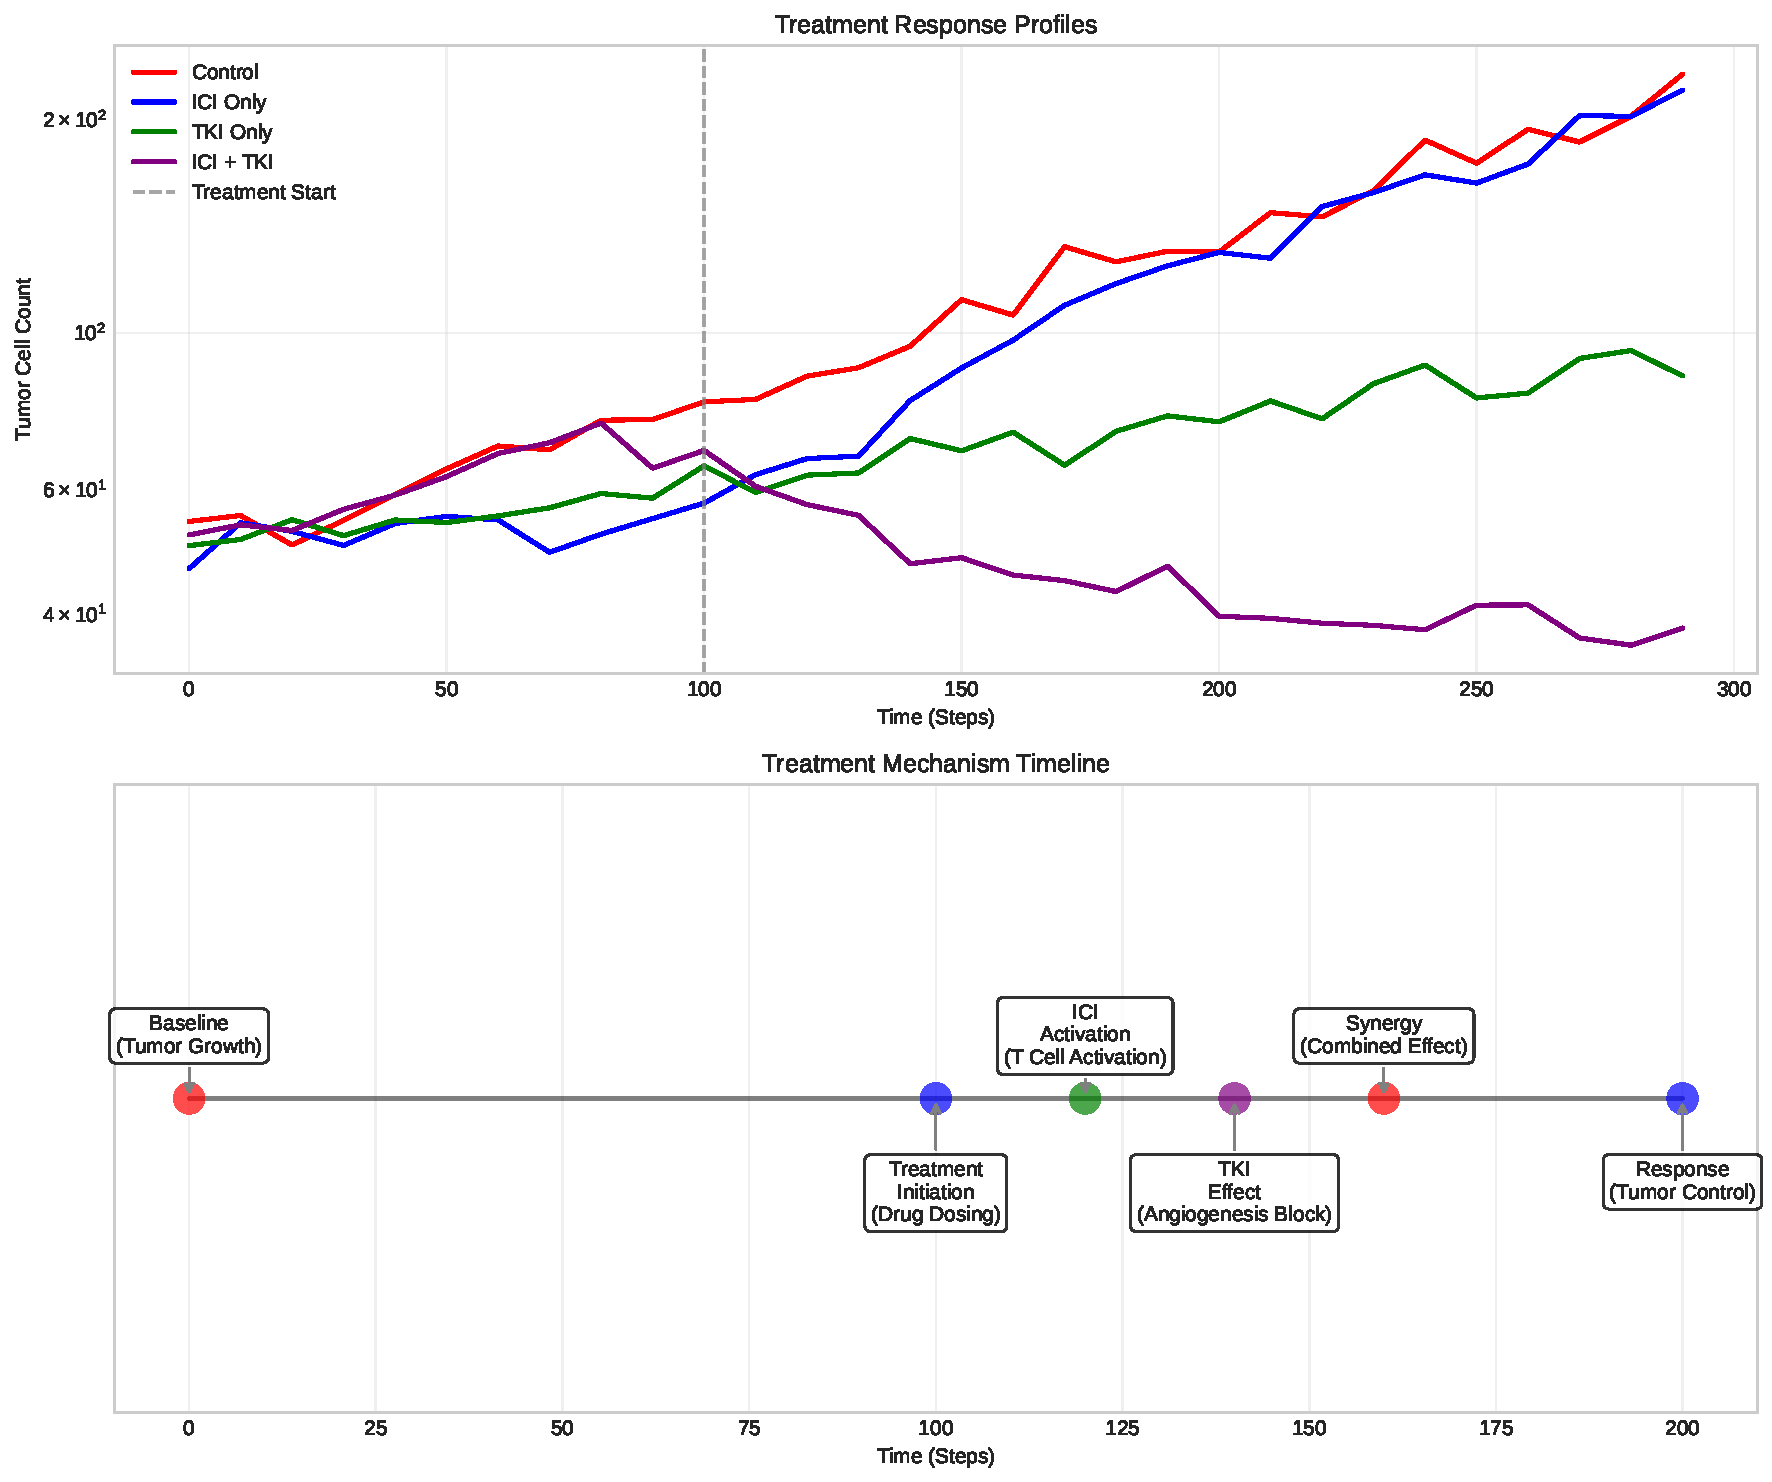
\includegraphics[width=0.85\textwidth]{figures/treatment_timeline.pdf}
\caption{Treatment timeline showing the sequential application of ICI and TKI therapies across simulation steps. The figure illustrates drug administration schedules, onset of action, and temporal coordination in combination therapy protocols.}
\label{fig:treatment_timeline}
\end{figure}

\begin{figure}[htbp]
\centering
\begin{tikzpicture}[
    node distance=1.5cm and 3.0cm,
    start/.style={ellipse, draw, fill=green!20, font=\small, minimum height=0.8cm, text width=1.8cm, text centered},
    decision/.style={diamond, draw, fill=orange!20, font=\scriptsize, minimum height=1.2cm, text width=1.8cm, text centered, inner sep=1pt, aspect=1.5},
    process/.style={rectangle, draw, fill=blue!15, font=\small, minimum height=1.0cm, text width=2.2cm, text centered, rounded corners=2pt},
    outcome/.style={rectangle, draw, fill=purple!15, font=\small, minimum height=1.0cm, text width=2.0cm, text centered, rounded corners=2pt},
    arrow/.style={->,>=stealth,thick}
]

% Start
\node[start] (start) {Treatment\\Decision};

% Main decision point
\node[decision, below=of start] (treat_type) {Treatment\\Type?};

% ICI Branch
\node[process, below left=of treat_type] (ici) {ICI\\Monotherapy};
\node[outcome, below=of ici] (ici_effect) {Block PD-1/PD-L1\\Restore T Activation};

% TKI Branch  
\node[process, below right=of treat_type] (tki) {TKI\\Monotherapy};
\node[outcome, below=of tki] (tki_effect) {Reduce Growth\\Release Neoantigens};

% Combination Branch
\node[process, below=of treat_type] (combo) {ICI + TKI\\Combination};
\node[outcome, below=of combo] (combo_effect) {Proportional\\Average (50/50)};

% No treatment branch
\node[process, left=of ici] (none) {No\\Treatment};
\node[outcome, below=of none] (none_effect) {Baseline\\Dynamics};

% Arrows
\draw[arrow] (start) -- (treat_type);
\draw[arrow] (treat_type) -- node[left, font=\scriptsize] {ICI} (ici);
\draw[arrow] (treat_type) -- node[right, font=\scriptsize] {TKI} (tki);
\draw[arrow] (treat_type) -- node[right, font=\scriptsize] {Combo} (combo);
\draw[arrow] (treat_type) -- node[above, font=\scriptsize] {None} (none);

\draw[arrow] (ici) -- (ici_effect);
\draw[arrow] (tki) -- (tki_effect);
\draw[arrow] (combo) -- (combo_effect);
\draw[arrow] (none) -- (none_effect);

% Additional annotations  
\node[font=\scriptsize] at ([xshift=1.5cm]ici_effect) {Immune Restoration};
\node[font=\scriptsize] at ([xshift=-1.5cm]tki_effect) {Anti-angiogenic + Immunogenic};  
\node[font=\scriptsize] at ([xshift=1.5cm]combo_effect) {Synergistic Mechanisms};

\end{tikzpicture}
\caption{Treatment Decision Flow showing the four treatment modalities available in the RCC model.}
\label{fig:treatment_decision_flow}
\end{figure}